\FloatBarrier
\section{Cache Performance of Odd-Even Merge Sort}
\label{sec:OEMergesortExperiment}

In Section~\ref{OEMergesortImpl} it is claimed that Odd-Even Mergesort benefits heavily from using an additional $\Theta(n)$ storage as a buffer to permute elements into a more memory-local ordering. Note that any efficient in-place permutation could easily replace this buffer, but efficient solutions for this problem do not appear immediately feasible.

Let us quickly reiterate what the problem is. Odd-Even Merging requires recursive calls to work on odd and even indices separately, which is often represented by providing a distance between elements to consider at the current level of the merge. This will however completely thrash the CPU cache by accessing elements in separate cache lines, leading to a massive performance degradation when data sizes grow beyond what fits into to last cache layer.
Swapping data back and forth between a buffer easily solves this problem, at the cost of a higher instruction count and memory usage.

Additionally, we have the opportunity to perform multiple layers of the recursive calls in each scan through the memory between each permuting step, which could lead to a reduction in cache misses.

The tests are performed in the same way as those of Section~\ref{sec:Performance}, but compares three executables, one using a buffer for Odd-Even Mergesort, one using a buffer and performing 2 layers of operation per re-ordering, and one having it disabled.

\subsection{Running Time and Cache Misses}

Figure~\ref{fig:Buffer:tc} shows the running time of the algorithm variants overlaid with the amount of cache misses per comparison performed. 
This shows a big difference in the amount of cache misses incurred between the buffered and unbuffered variants, and highlights the corresponding increase in running time for the unbuffered version of Odd-Even Mergesort. 
Note that the increase in running time makes the algorithm grow asymptotically faster than $O(n \log^2 n)$ for inputs larger than the CPU cache, while the buffered variants shows a running time that is much more consistent with the running time suggested by the standard RAM model.
There seems to be almost no difference in running time between the single-layered and double-layered buffering variants.

\begin{figure}
\center
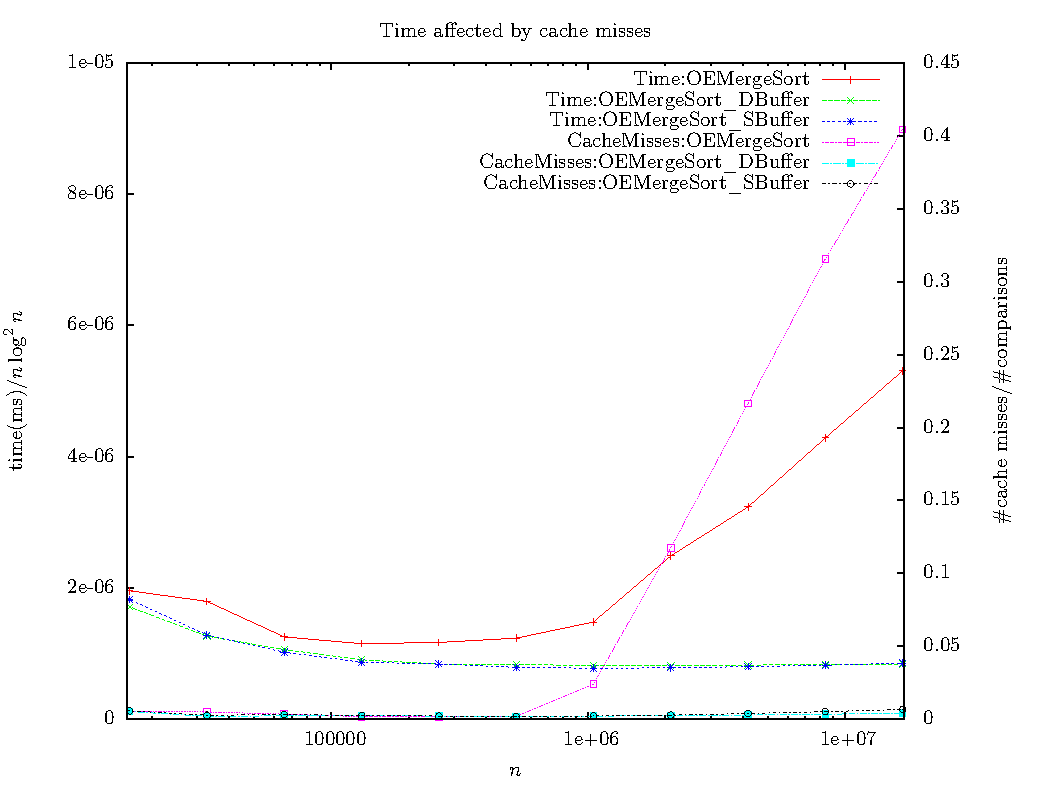
\includegraphics[width=\textwidth]{graphs/Buffer/tc.pdf}
\caption{Time overlaid with cache misses}
\label{fig:Buffer:tc}
\end{figure}


When looking at Figure~\ref{fig:Buffer:tc}, it is also clear that the unbuffered variant of Odd-Even Mergesort grows faster than $O(n \log^2 n)$ even for values well within the cache limit.
This observation might seem strange at first, but Figure~\ref{fig:Buffer:tc2} will show a reasonable explanation for this being the L1 cache layer. In the aforementioned figure, we can see the running time overlaid with the amount of L1 cache load misses. The L1 cache is much smaller than the total CPU cache, and the latency between L1 and the outer cache layer is much smaller than the main memory latency, but still significant. We see that the unbuffered variant of Odd-Even Mergesort incurs  a lot more L1 load misses, which will unfavourable affect running time, and helps explaining why it is slower, even within cache limits.

The single-layered and double-layered variants show a significant difference in L1 cache load misses, but not much of a difference in running time. This is caused by the extra complexity required to compute the double-layered indices counter-acting the performance gained from a slightly reduced number of L1 cache misses.

\begin{figure}
\center
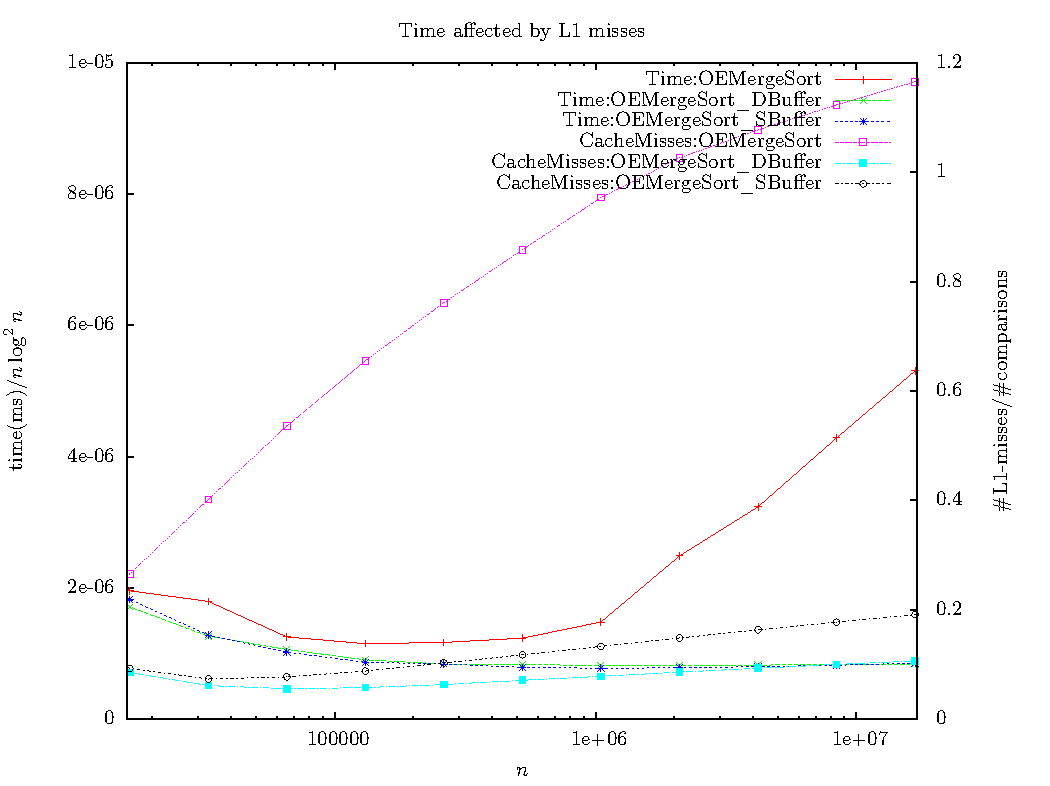
\includegraphics[width=\textwidth]{graphs/Buffer/tc2.pdf}
\caption{Time overlaid with cache misses}
\label{fig:Buffer:tc2}
\end{figure}


\subsection{Experiment Results}

The experiment show that moving data around in preparation to the recursive calls of the Odd-Even Merging does indeed have a large and measurable effect on performance. This shows that one must take care when implementing sorting networks directly on the CPU and justifies our solution of using buffers. 
Additionally, we can see that the two-layered cache-reordering strategy is feasible, but is not much better than performing a single layer per reordering. The lower amount of L1 cache misses, combined with an almost identical running time makes it favourable, but this might change depending on the development in cache speed versus instruction speed. 
